\section{Changing the direction of a test}\label{sec:switching}

Fix one stage and orient the preceding color toward the west as in
Section~\ref{sec:probability}. To extend the coverage bound \(t\) to
the larger cluster, we must choose a direction for each refined color.
The choice depends on the cuts covering the west test. If their total
weight on a suitable list is small, we keep testing west. If the
weight is large, we switch east.

Two facts make the switch possible. First, only a small weight of
west cuts can also be charged along the east spine. Most cuts can
therefore be carried forward along that spine. Second, among the cuts
that persist, one can select a cut \(D\) and many newer cuts whose keys
all strictly reach those of \(D\) (Lemma~\ref{lem:good-comparisons}).
An east test that succeeds must pass barrier bits shared by the newer
cuts. Except on a rare event, it must also succeed from a key of \(D\),
where none of those bits can be read. Their independence gives a
contraction for east coverage.

\subsection{Cuts hit by both spines}

The first refinement appends \(h\) scale bits to the old color of a
micro node. We call the result its \emph{mid color}. Compute the bits
at the node's east key \(v\), using the old-color core list at \(v\)
of depth \(4H\). For each \(s=a^j\), \(0\le j<h\), collect the cuts
\(B\) on this list for which some east-spine charge at a site \(x\)
satisfies
\begin{equation}\label{eq:scale-bit}
 s\le x-l(B)<as,\qquad x-m(v)\le s/10 .
\end{equation}
Set the bit if these cuts have total weight at least
\(\theta=t a^{-10K}\). The charge at \(x\) need not be the first one
to \(B\). Thus the bit records a large collection of cuts of span
comparable to \(s\), each charged within \(s/10\) of the observation
site. Put \(f_*=(3K+6)H\).

The two occurrences of a mid color in Figure~\ref{fig:cut-transfer}
read the same scale bit. This will force an older cut to acquire an
east charge near the left endpoint of a newer one.

\begin{figure}[htbp]
\centering
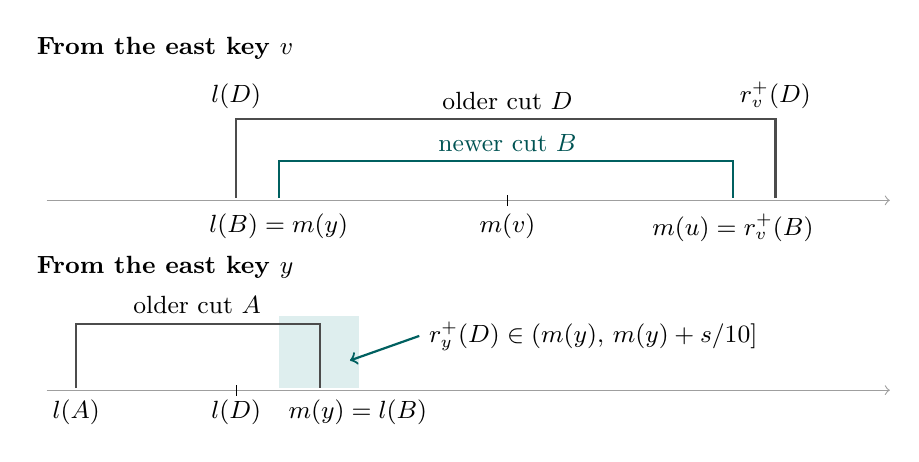
\begin{tikzpicture}[x=.83cm,y=.82cm,font=\small,
    axis/.style={->,gray!75},older/.style={draw=black!70,thick},
    newer/.style={draw=teal!75!black,thick}]
  \node[anchor=west,font=\small\bfseries] at (0,2.72) {From the east key \(v\)};
  \draw[axis] (.3,.36)--(13.2,.36);
  \draw[older] (3.2,.4)--(3.2,1.62)--(11.45,1.62)--(11.45,.4);
  \node[above] at (3.2,1.62) {\(l(D)\)};
  \node[above] at (7.35,1.62) {older cut \(D\)};
  \node[above] at (11.45,1.62) {\(r_v^+(D)\)};
  \draw[newer] (3.85,.4)--(3.85,.97)--(10.8,.97)--(10.8,.4);
  \node[above,text=teal!65!black] at (7.35,.97) {newer cut \(B\)};
  \draw (7.35,.27)--(7.35,.45);
  \node[below] at (3.85,.3) {\(l(B)=m(y)\)};
  \node[below] at (7.35,.3) {\(m(v)\)};
  \node[below] at (10.8,.3) {\(m(u)=r_v^+(B)\)};

  \node[anchor=west,font=\small\bfseries] at (0,-.68) {From the east key \(y\)};
  \draw[axis] (.3,-2.58)--(13.2,-2.58);
  \fill[teal!13] (3.85,-2.55) rectangle (5.08,-1.43);
  \draw[older] (.75,-2.55)--(.75,-1.55)--(4.48,-1.55)--(4.48,-2.55);
  \node[above] at (2.60,-1.55) {older cut \(A\)};
  \draw (3.2,-2.67)--(3.2,-2.5);
  \node[below] at (.75,-2.58) {\(l(A)\)};
  \node[below] at (3.2,-2.58) {\(l(D)\)};
  \node[below,anchor=north west] at (3.85,-2.58) {\(m(y)=l(B)\)};
  \node[anchor=west] (window) at (6,-1.74)
    {\(r_y^+(D)\in(m(y),\,m(y)+s/10]\)};
  \draw[newer,->] (window.west)--(4.94,-2.12);
\end{tikzpicture}
\caption{Transferring an endpoint. At \(v\), the first east charge
to \(B\) occurs at \(u\). Older cuts such as \(D\) set the scale bit
there. A west flag witness for \(B\) carries that same bit to \(y\).
At \(y\), the bit supplies a cut \(A\) with an old charge in the
shaded interval. Now \(D\) is newer than \(A\), forcing a mid charge
to \(D\) in that interval. Positions are schematic.}
\label{fig:cut-transfer}
\end{figure}

\begin{lemma}[Cuts charged by both spines]\label{lem:straddlers}
On the mid-color core list of depth \(f_*\) at any east key \(v\),
the cuts with \(r_v^+(B)<\infty\) have total weight at most \(t/a\).
\end{lemma}

\begin{proof}
Suppose the finite-endpoint cuts have weight greater than \(t/a\).
Starting at \(v\), we pass to another east key and retain a subfamily
of these cuts. Each step spends \(3H\) of depth and retains at least
\(a^{-4}\) of the weight. Every retained cut has a strictly smaller
finite right endpoint at the new key. This last property prevents
\(K\) such steps, since a cut has at most \(K\) keys.
Before each step we thus have \(f\ge9H\) and weight
\(M\ge t a^{-1-4(K-1)}\).

\emph{Selecting a nested pair.}
Group the cuts by the scale \(s\le r_v^+(B)-l(B)<as\), then by
the bins of width \(s/10\) containing their two endpoints. All these
intervals straddle \(m(v)\), so there are \(O_h(a^2)\) groups. One has
weight \(M'\ge c_h M/a^2\). Write \(\beta=t^2a^{-100K}\). The
bad ordered pairs in this group have product weight at most \(\beta\)
by Lemma~\ref{lem:good-comparisons}. Both orientations of a good
pair have the same product weight. Averaging, some cut \(B\) is
newer than cuts \(D\) of total weight at least
\((M'^2-\beta)/(2M')\ge M'/3\).

\emph{Reading the bit on the east.}
Let \(u\) be the east key at the first charge to \(B\) on the east
spine from \(v\). Every one of these older cuts \(D\) covers the
mid-color west test at \(u\) to depth \(f-H\), by
Lemma~\ref{lem:good-comparisons}. It therefore covers the old test
to depth \(4H\). Indeed each old path is allowed in the mid round,
and every mid charge on it is an old charge. By
Lemma~\ref{lem:proper-loss} applied between the list at \(v\) and the
old tests at \(u\), discard weight at most \(E_0\) to ensure
that no proper subset covers the old test at \(u\) to depth \(H_-\).
Since \(H_-<H\), this gives minimality at depth \(H\) as well. The
old and mid lists use the same requirement of possible screened
success for the keys of \(D\). Each remaining \(D\) therefore belongs
to the old core list at \(u\). Its former right endpoint occurs strictly
after \(u\) as an old charge on the continuing east spine. The common
right-endpoint bin and the choice of scale give
\eqref{eq:scale-bit}. The remaining mass exceeds \(\theta\).
Consequently the bit for \(s\) is set at \(u\), and the flag witness
for this charge to \(B\), which has east key \(u\), shows that the
bit is set in the given mid color.

\emph{Transporting the bit to the west.}
Take a mid west path at \(v\) witnessing the necessity, to depth
\(H\), of a west key of \(B\) at site \(l(B)\). At its first charge
to \(B\), go to the flag witness for this charge, and from the witness
move to its \emph{east} key \(y\). Thus \(m(y)=l(B)\). No older \(D\)
can have been charged before the first \(B\) charge, by the proof of
Lemma~\ref{lem:good-comparisons}. Going to the witness charges at most
the same west key of \(B\). For the move to \(y\), discard cuts
containing \(y\), of weight at most \(2p\) by
Lemma~\ref{lem:cut-list}. The prefix to \(y\) uses at most \(H+1\)
moves per site. Prepending it shows that the remaining \(D\)'s cover
mid west tests at \(y\) to depth \(f-3H\), and hence cover the old
tests there as well. By another application of
Lemma~\ref{lem:proper-loss} from \(v\) to \(y\), discard weight at most
\(E_0\) to ensure minimality to depth \(H\) in the old round. This
implies minimality in the mid round, since any covering subset in the
mid round covers the old tests. We have placed these cuts on the mid
core list at \(y\) of depth \(f-3H\) and the old one of depth \(4H\).

\emph{Forcing a new east endpoint.}
The witness at the west endpoint has the same mid color as the east
witness. Thus
the bit for \(s\) is set at its east key \(y\). At \(y\) the old list
contains cuts \(A\) of weight at least \(\theta\) charged at
\(x\le m(y)+s/10\) with \(l(A)\le m(y)-9s/10\).
By the product-weight bound on this old list, except for cuts \(D\)
of total weight at most \(\beta/\theta\), each transferred \(D\) has
a good comparison with such an \(A\). Since
\(\lvert l(D)-m(y)\rvert\le s/10\), \(l(D)>l(A)\).
Thus \(D\) has changed roles. At \(v\) it was older than \(B\).
At \(y\) it is newer than \(A\), so every key of \(D\) strictly
reaches the nearby key of \(A\).

The comparison at \(y\) was made in the old round. To finish the step
we need a \emph{mid} charge to \(D\) on the east spine from
\(y\) by site \(m(y)+s/10\). Otherwise follow the basic spine to
the east key \(g\) of the indicated old charge to \(A\).
That prefix misses \(D\) in the mid round. It uses at most three
moves per site, so \(D\) transfers to \(g\), covering even the old
west test to depth \(H\). Since \(g\in A\) and \((D,A)\) is good in
the old list, no proper subset of \(D\) covers that test even to
depth \(H_-\). Minimality forces \(g\) to reach every key of \(D\).
But every key of \(D\) strictly reaches \(g\) by the same comparison,
contradicting acyclicity.

The accumulated losses \(2E_0+2p+\beta/\theta\) are \(o(M')\),
and \(M'/3-o(M')\ge M/a^4\) for large \(a\). The new finite right
endpoint of every retained \(D\) is at most \(m(y)+s/10\), whereas
its former one was greater than \(r_v^+(B)\ge m(y)+s\). This proves
the asserted step. After \(K\) steps a retained cut would have had
\(K+1\) distinct right endpoints, each the site of one of its at most
\(K\) keys.
\end{proof}

\subsection{The direction and its barrier bits}

When the start moves east from \(v\) to \(u\), we transfer a west test
at \(u\) back to \(v\) by prepending the intervening spine. The
following depth vector saves four moves per visited site for exactly
that purpose. Define the \emph{band list} at an east key \(v\) to be
its mid-color core list with depth vector
\[
 F_v=f_*+(K+5)d+\sigma_v,\qquad
 \sigma_v(x)=
 \begin{cases}
 0& x<m(v),\\
 4& x=m(v),\\
 8& x>m(v).
 \end{cases}
\]
Compute the next refinement of a micro node at its east key \(v\).
If the total band weight is less than \(t/4\), append the symbol
\emph{neutral} and keep the west direction. Otherwise append the
unique \(b=(t/4)2^j\), \(j\ge0\), for which that weight lies in
\([b,2b)\), and set the direction east. In the latter case the gate
at this east key in this new color requires one additional bit for
each \(B\) on its band list. The bit is shared by all such gates
within the stage and new color that require it. Its index consists
of the stage, the new color, and \(B\). Choose its success
probability, depending only on the parameters, \(b\), and \(|B|\),
rationally in the interval
\[
 [\exp(-2\lambda r(B)/b),\,\exp(-\lambda r(B)/b)] .
\]
These are the only new barrier requirements. At any one key their
joint passage probability is at least \(\exp(-4\lambda)\). A new
gate requires the screened old gate, its fresh independent
key-thinning bit of probability \(z\), and the barriers just assigned.

Lemma~\ref{lem:cut-list} bounds every band weight by \(aU\), so there
are \(O(\log a)\) bins. With \(h\) fixed, the \(h\) scale bits and the
bins at each of the \(h-1\) refinement stages give polylogarithmically
many colors. The rules are local. A depth bound \(F\) gives a radius
at most \(L_0\max_x F(x)\), and minimality makes every cut key
reachable within such a bound. Coverage, possibility, and all
probabilities defining a screen can be evaluated from the resulting
finite unfoldings and the local rules of the preceding stages.

\subsection{The probability bound in the new direction}

We now relate the two deterministic lists used by the color rule to
the probability of coverage by successful gates. Three steps suffice.
Coverage after thinning usually produces a core cut of at most \(K\)
successful keys. Lemma~\ref{lem:two-spine-estimates} uses that cut to
bound the exceptional west tests. Proposition~\ref{prop:directional-cap}
then uses the shared barriers to obtain the cap after switching east.

Fix the mid color. Throughout, arbitrary sites may be ignored and
the raw bits there fixed arbitrarily. Count only hits at other sites.
Call a key \emph{thinned} here if its screened old gate and its new
thinning bit both succeed. Write \(f^\sharp=f+(K+4)d\), also for a
depth vector, with addition in each component.

\begin{lemma}[Extracting a cut after thinning]\label{lem:thinned-cover}
Let \(v\) be an east key and \(f\ge f_*\) a depth used in this stage.
Except on an event of probability \(o(t)\), mid west coverage at
\(v\) by thinned keys to depth \(f^\sharp\) implies that a cut on the
mid core list of depth \(f\) consists of nonignored thinned keys.
The error is uniform under the allowed conditioning.
\end{lemma}

\begin{proof}
Expose all bits through the preceding stage. Carry out the branching
search of Lemma~\ref{lem:cut-list} among the screened successes at
nonignored sites, stopping a branch when it covers to depth
\(f^\sharp-d\). Before it stops, any extension covering to depth
\(f^\sharp\) must use one of the \(a^{o(1)}\) candidates at its next
step. The candidates depend only on the exposed randomness. If
coverage by thinned keys occurs, follow only branches whose selected
keys survive thinning. Either one stops early or one reaches \(K\)
distinct surviving keys. Coverage also requires coverage in the crude
old test, an event of probability at most \(U\) measurable before
thinning. Thus the latter possibility together with coverage has
probability at most
\[
 Ua^{o(1)}z^K=o(t).
\]

On an early stopping branch the selected keys cover to depth
\(f^\sharp-d\). The minimum sizes of covering subsets of these keys
at depths \(f,f+d,\ldots,f+(K+2)d\) are nondecreasing integers in
\([1,K]\). Two consecutive values agree. A minimum subset at the
larger depth is minimal at the smaller, so belongs to the corresponding
two-depth mid list. If it fails to be minimal at depth \(H\), it has
a proper subset covering to \(H_-\). For each of the \(K+2\) possible
lists Lemma~\ref{lem:proper-loss} bounds the weight lost this way by
\(E_0\). A fixed cut of nonignored keys succeeds with probability at
most its weight, since it requires its independent pins. This adds
only \(O(KE_0)=o(t)\). Every remaining cut belongs to the claimed
core list.
\end{proof}

The two parts of the following lemma will bound coverage for the
neutral and switched colors, respectively.

\begin{lemma}[Coverage on the two spines]\label{lem:two-spine-estimates}
At every east key \(v\) the following estimates hold.
\begin{enumerate}
\item\label{item:small-band}
If \(v\) gives the neutral refinement, mid west coverage to
\((F_v)^\sharp\) by thinned keys has probability at most \(t/4+o(t)\).
\item\label{item:rare-joint-hit}
The probability of mid west coverage to \((f_*)^\sharp\) by thinned
keys \emph{and} a mid charge to a nonignored thinned key on the east
spine is \(o(t)\).
\end{enumerate}
\end{lemma}

\begin{proof}
The first estimate follows by the band weight and Lemma~\ref{lem:thinned-cover}.
For the second estimate, Lemma~\ref{lem:thinned-cover} provides a
successful cut \(B\) of depth \(f_*\), and Lemma~\ref{lem:straddlers}
costs at most \(t/a\) for cuts that meet the east spine. Otherwise
let the spine reach the charged thinned key \(g\). The screen at
\(g\) gives a missed old west path at depth \(d\) ignoring its site.
Prepend the east spine to \(g\). The concatenation is a mid west test
at \(v\) to depth \(f_*\), so must charge \(B\). All keys of \(B\) have
successful old gates. The hit must therefore be a key of \(B\) at
\(g\)'s site, distinct from \(g\). For fixed \(B\) there are at most
\(K\) candidate sites for \(g\) and at most one charged spine key at
each. At nonignored sites the additional pin is independent, so the
joint probability is at most \(Kp\,r(B)\). Summing gives at most
\(KpaU=o(t)\).
\end{proof}

\begin{proposition}[Coverage after one refinement stage]\label{prop:directional-cap}
For some \(D_i=O(D_{i-1}\log a)\), each new color has coverage
probability at most \(t\) in its chosen direction from every node
of its cluster, under arbitrary allowed conditioning on ignored sites.
\end{proposition}

\begin{proof}
For a neutral new color, test west from an arbitrary node. Follow its
west spine to the first charge in that color, go to its flag witness,
and from there to its east key \(v\), which gives the neutral
refinement. If there is no charge, coverage is impossible. The prefix
is deterministic, uses at most four moves per site, and has at most
two possible charges to nonignored keys in the new color. It has a
successful such charge with probability at most \(2p\). Otherwise
coverage at the starting node forces new west coverage at \(v\)
with the depth decreased by four, and hence mid west coverage there
by thinned keys. With starting depth at least
\(\max_x (F_v)^\sharp(x)+4\), Lemma~\ref{lem:two-spine-estimates}(\ref{item:small-band}) proves the
desired cap \(t\).

Consider finally a new color with bin \(b\), and an east key \(v\)
giving that refinement. Let \(\mathcal D\) be the intersection of the
band lists for the mid color over all east keys along the east spine
from \(v\), including \(v\). We claim
\begin{equation}\label{eq:common-bands}
 \sum_{B\in\mathcal D}r(B)\ge 0.9b .
\end{equation}
At \(v\) discard the cuts hit by that spine, of weight at most \(t/a\)
by Lemma~\ref{lem:straddlers}, since its band list is contained in
the core list at \(f_*\). For any later east key \(u\) on the spine,
prepend the spine prefix. It uses at most three moves per site, and
at each site used \(F_v(x)-F_u(x)\ge4\). Thus each retained cut
covers to \(F_u\) at \(u\). At the \emph{last} such east key discard
weight at most \(E_0\) by Lemma~\ref{lem:proper-loss} to guarantee
minimality to depth \(H_-\) there. From each earlier east key prepend
the segment to the last key to each witness of minimality. The segment
misses the cut and \(H_-+3\le H\), so this establishes minimality to
depth \(H\) at every one of them. A single application of the loss
bound therefore suffices to prove \eqref{eq:common-bands}.

By the good-pair averaging argument in Lemma~\ref{lem:straddlers},
applied now to the older member, there is \(D\in\mathcal D\) and
there are \(B\in\mathcal D\) newer than \(D\) of weight at least
\(b/4\). All of their corresponding barrier bits pass with probability
at most \(e^{-\lambda/4}\). A coverage test at \(g\in D\) uses only random bits indexed by
reachable keys or by sets of reachable keys. Every key of a newer
\(B\) strictly reaches \(g\), so acyclicity prevents \(g\) from
reaching any of them. The shared barrier bit indexed by \(B\)
is therefore independent of the coverage event at \(g\). This
independence also holds after the permitted conditioning on raw bits.

Suppose there is new east coverage at \(v\) to depth \(R>F_{\max}\),
where \(F_{\max}=f_*+(K+5)d+8\). The east spine must charge a successful
new gate. The charge has a flag witness of this new color with the
same east key. Hence that key assigns the bin \(b\) and requires
every shared barrier above. If thinned keys also cover the mid west
tests at \(v\) to depth \(F_v\), Lemma~\ref{lem:two-spine-estimates}(\ref{item:rare-joint-hit}) bounds this case by \(o(t)\), since
\(F_v\ge(f_*)^\sharp\) and the successful east charge is also a
thinned mid charge. Otherwise choose a missed mid west path to depth
\(F_v\). As \(D\) belongs to the band list, this path charges some
key \(g\in D\). Redirect this move to \(g\) itself. The prefix uses
allowed new moves, and every new charge is also a mid charge, so it
contains no nonignored successful new charge. It follows by
concatenation that new east coverage to depth \(R-F_{\max}\) must
hold at \(g\).

Let \(\Pi(R)\) be the supremum of new east coverage probabilities
over starting nodes in the cluster for this new color and the given
conditioning. From an arbitrary starting node use the east spine
up to its first new charge and go to its east key, which assigns
this bin by the flag witness. The prefix uses at most four moves per site. Its possible charged
keys are determined by the flags, before any random bits are read.
The probability of a nonignored success on the prefix is at most
\(2p\). Using the preceding implication at
that key, independence of the shared barriers, and a union bound
over the fixed set \(D\), we obtain
\[
 \Pi(R+4)\le o(t)+K e^{-\lambda/4}\Pi(R-F_{\max}).
\]
The coefficient \(\rho=K e^{-\lambda/4}\) is less than \(1/4\).
Start with the bound \(\Pi\le1\) and iterate
\(k=\lceil2J\log_2 a\rceil\) times. The contribution \(\rho^k\)
is at most \(a^{-4J}=t^4\), and the uniform errors sum to
\(o(t)/(1-\rho)=o(t)\). Thus \(\Pi\le t\) for large \(a\). A common depth \(D_i=O(D_{i-1}\log a)\) meets this
bound and the neutral one. Since \(h\) is fixed, every stage has
\(D_i=a^{o(1)}\). This completes the induction.
\end{proof}

\subsection{The last screen}

After stage \(h-1\), merge once more to the full interval. Set
\(d=D_{h-1}\). At depth \(d\) the crude cap \(U\) now applies to
coverage of all paths to leaves, since there are no exits. For each
key and color add a final screen forbidding this coverage with the
key's own site ignored. The resulting gate will be called final.

\begin{lemma}[A final gate and its continuation]\label{lem:final-gates}
For every key \(g\) and final color, its required raw bits have joint
success probability at least \(q^{-2}\), and its required barriers
have joint passage probability at least \(\exp(-4h\lambda)\).
Condition on the required raw successes at \(g\), optionally also
at one other key of the same site. The sum of the conditional
failure probabilities of its required screens is \(o(1)\), uniformly
over the allowed graphs and choices. Whenever the final gate at
\(g\) succeeds, there is a path from \(g\) to a leaf of per-site depth
at most \(d\) on which every charge to a successful final gate in
this color lies in the site of \(g\).
\end{lemma}

\begin{proof}
The raw probability is at least \(q^{-1}z^h=q^{-2}\). All barriers
ask for successes of deterministic sets of independent bits, so
multiplying their per-stage lower bounds gives the stated estimate.
For the screen of a given stage, later raw bits can be dropped from
the conditioning. Every subset of the remaining one or two pins is
in the key's site. The ignored-site crude cap gives conditional
coverage probability at most \(U\) under each such subset, so
Lemma~\ref{lem:pcost} gives conditional screen cost \(o(1)\).
The final screen costs at most \(U\) by the same crude cap. There
are at most \(h\) screens. Passage of the last one provides the
asserted path, since final successes are among the gate successes
tested by that screen.
\end{proof}
